%%%%%%%%%%%%%%%%%%%%%%%%%%%%%%%%%%%%%%%%%
% Beamer Presentation
% LaTeX Template
%
% This template has been downloaded from:
% http://www.LaTeXTemplates.com
%
% This template has been altered after it was downloaded from the 
% above link
%
% License:
% CC BY-NC-SA 3.0 (http://creativecommons.org/licenses/by-nc-sa/3.0/)
%
%%%%%%%%%%%%%%%%%%%%%%%%%%%%%%%%%%%%%%%%%

%----------------------------------------------------------------------------------------
%	PACKAGES AND THEMES


\documentclass{beamer}

\mode<presentation> {

% The Beamer class comes with a number of default slide themes
% which change the colors and layouts of slides. Below this is a list
% of all the themes, uncomment each in turn to see what they look like.

%\usetheme{default}
%\usetheme{AnnArbor}
%\usetheme{Antibes}
%\usetheme{Bergen}
%\usetheme{Berkeley}
%\usetheme{Berlin}
\usetheme{Boadilla}
%\usetheme{CambridgeUS}
%\usetheme{Copenhagen}
%\usetheme{Darmstadt}
%\usetheme{Dresden}
%\usetheme{Frankfurt}
%\usetheme{Goettingen}
%\usetheme{Hannover}
%\usetheme{Ilmenau}
%\usetheme{JuanLesPins}
%\usetheme{Luebeck}
%\usetheme{Madrid}
%\usetheme{Malmoe}
%\usetheme{Marburg}
%\usetheme{Montpellier}
%\usetheme{PaloAlto}
%\usetheme{Pittsburgh}
%\usetheme{Rochester}
%\usetheme{Singapore}
%\usetheme{Szeged}
%\usetheme{Warsaw}

% As well as themes, the Beamer class has a number of color themes
% for any slide theme. Uncomment each of these in turn to see how it
% changes the colors of your current slide theme.

%\usecolortheme{albatross}
%\usecolortheme{beaver}
%\usecolortheme{beetle}
%\usecolortheme{crane}
%\usecolortheme{dolphin}
%\usecolortheme{dove}
%\usecolortheme{fly}
%\usecolortheme{lily}
%\usecolortheme{orchid}
%\usecolortheme{rose}
\usecolortheme{seagull}
%\usecolortheme{seahorse}
%\usecolortheme{whale}
%\usecolortheme{wolverine}

% Here is an overview of possible theme and colortheme combinations:
% https://hartwork.org/beamer-theme-matrix/

%\setbeamertemplate{footline} % To remove the footer line in all slides uncomment this line
%\setbeamertemplate{footline}[page number] % To replace the footer line in all slides with a simple slide count uncomment this line

\setbeamertemplate{navigation symbols}{} % To remove the navigation symbols from the bottom of all slides uncomment this line
}

\usepackage{graphicx} % Allows including images
\usepackage{booktabs} % Allows the use of \toprule, \midrule and \bottomrule in tables
\usepackage{appendixnumberbeamer} % Allows use of \appendix. Slides appearing after will not be part of the frame counter or navigation panel
\usepackage{todonotes} % Allows use of \missingfigure

\usepackage{mathtools}

\newcommand\blfootnote[1]{%
	\begingroup
	\renewcommand\thefootnote{}\footnote{#1}%
	\addtocounter{footnote}{-1}%
	\endgroup
}

% Following lines makes a section overview at the beginning of each section 
\setbeamertemplate{caption}{\raggedright\insertcaption\par}
\AtBeginSection[]
{
 \begin{frame}<beamer>
 %\frametitle{Plan}
 \tableofcontents[currentsection]
 \end{frame}
}

%----------------------------------------------------------------------------------------
%   TITLE PAGE
%----------------------------------------------------------------------------------------

\title[Week 7]{Graph-CSPNet} % The short title appears at the bottom of every slide (dependent on theme), the full title is only on the title page

\author{Artyom Matveev} % Your name
\institute[MIPT] % Your institution as it will appear on every slide (dependent on theme), may be shorthand to save space
{
Moscow Institute of Physics and Technology \\ % Your institution for the title page
\medskip
\textit{matveev.as@phystech.edu} % Your email address
}
\date{November 11, 2023} % Date, can be changed to a custom date

\begin{document}

{
%\usebackgroundtemplate{\includegraphics[width=\paperwidth]{figures/background.jpg}} % background of first slide
\begin{frame}
\titlepage % Print the title page as the first slide
\end{frame}
}

%\begin{frame}
%\frametitle{Overview} % Table of contents slide, comment this block out to remove it
%\tableofcontents % Throughout your presentation, if you choose to use \section{} and \subsection{} commands, these will automatically be printed on this slide as an overview of your presentation
%\end{frame}

%----------------------------------------------------------------------------------------
%   PRESENTATION SLIDES
%----------------------------------------------------------------------------------------

%------------------------------------------------
%\section{First Section} % Sections can be created in order to organize your presentation into discrete blocks, all sections and subsections are automatically printed in the table of contents as an overview of the talk
%%------------------------------------------------
%
%\subsection{Subsection Example} % A subsection can be created just before a set of slides with a common theme to further break down your presentation into chunks

\begin{frame}{Model's structure%
		\setcounter{footnote}{0}\footnotemark}
%\frametitle{Model's structure}

\stepcounter{footnote}
\footnotetext{\tiny{\textbf{Ju, C.}, \& Guan, C. Graph Neural Networks on SPD Manifolds for Motor Imagery Classification: A Perspective From the Time–Frequency Analysis. IEEE Transactions on Neural Networks and Learning System. 2023}}

\begin{enumerate}
\item SPDNet\footnote{\tiny{\textbf{Huang, Z.}, \& Van Gool, L. A Riemannian Network for SPD Matrix Learning. AAAI-2017}}. A neural network that operates on SPD matrices.
\begin{itemize}
	\item BiMap layer. It transforms the input SPD matrices to new SPD matrices by a bilinear mapping.
	\item ReEig layer. It rectifies the SPD matrices by tuning up their small positive eigenvalues.
	\item LOG layer. It maps an SPD matrix $\mathbf{S}$ onto its tangent space at identity matrix $\mathbf{I}$.
\end{itemize}

\item Riemannian Batch Normalization\footnote{\tiny{\textbf{Brooks, D.}, Schwander, O., et al. Riemannian batch normalization for SPD neural networks. NeurIPS 2019}}.

%\begin{center}
%	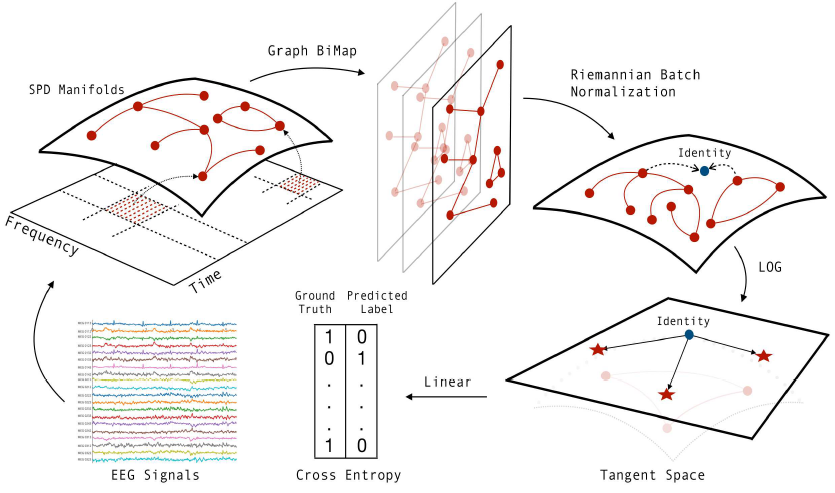
\includegraphics[height = 3.5cm, width=6.5cm]{images/2023_Ju.png}
%\end{center}
\end{enumerate}

%\blfootnote{\tiny{\textbf{Barachant, A.}, Bonnet, S., et al. Multiclass brain-computer interface classification by Riemannian geometry. 2012}}
\end{frame}

%------------------------------------------------

\begin{frame}
\frametitle{Graph construction}
\begin{enumerate}
\item $\mathbf{X} \in \mathbb{R}^{n_C \times n_T}$ -- an EEG signals trial

\item $\mathbf{S} = \mathbf{X} \mathbf{X}^{\top} \in \mathcal{S}_{++}$ -- an SPD matrix

\item $\mathbf{S} = \mathbf{U} \mathbf{\Sigma} \mathbf{U}^{\top}$ -- an SPD matrix representation using eigenvalue decomposition

\item $d_{g^{\text{AIRM}}} (\mathbf{S}_1, \mathbf{S}_2) = d_{g^{\text{AIRM}}} (\mathbf{W} \mathbf{S}_1 \mathbf{W}^{\top}, \mathbf{W} \mathbf{S}_2 \mathbf{W}^{\top})$, where $\mathbf{W}$ is weight matrix of BiMap transformation \underline{with the full-row rank}

\item $\mathcal{G} = (\mathcal{V}, \mathcal{E})$ -- a time-frequency graph:
\begin{itemize}
	\item $\mathcal{V}(\mathcal{G}) \coloneqq \{\mathbf{S}_i = S(\Delta t_i \times \Delta f_i)\}$, where $\{S(\Delta t_i \times \Delta f_i)\}_{i \in \mathcal{I}}$ is the set of SPD matrices under the specific time and frequency constraints.
	
	\item \[
			\mathcal{E}(\mathcal{G}) \coloneqq \mathbf{A} =
			\begin{cases}
				e^{-d^2_{g^{\text{AIRM}}} (\mathbf{S}_i, \mathbf{S}_j) / t}, & \text{if $\mathbf{S}_i$ and $\mathbf{S}_j$ are adjacent} \\
				0, & \text{others}
			\end{cases}
		  \] where $e^{(\cdot)}$ is the RBF kernel and preset Gaussian kernel width $t > 0$.
\end{itemize}
\end{enumerate}
\end{frame}

%------------------------------------------------

\begin{frame}
\frametitle{Graph BiMap Layer}

Each GNN layer updates the following way:

\[
	H^{(l+1)} \leftarrow \text{RBN}\left(\text{ReEig}\left(\mathbf{W}^{(l)}(\mathbf{\bar{D}}^{-1} \mathbf{\bar{A}}^{(l)}) H^{(l)} \mathbf{W}^{(l) ^ \top}\right)\right),
\]
where $\mathbf{\bar{A}}^{(l)} \coloneqq \mathbf{A}^{(l)} + \mathbf{I}_N$, $\mathbf{\bar{D}}_{ii} \coloneqq \sum_j \mathbf{\bar{A}}^{(l)}_{ij}$, $H^{(l)} \in \mathbb{R}^{\lvert \mathcal{V} \rvert \times n_C^2}$, $\mathbf{\bar{A}}^{(0)}$ is the adjacency matrix of the time-frequency graph, and $\mathbf{\bar{A}}^{(l)} \coloneqq \mathbf{I}_N$, for $l \ge 1$.

\begin{block}{ReEig layer}
	This layer performs $\mathbf{U} \max(\epsilon \mathbf{I}, \mathbf{\Sigma}) \mathbf{U}^{\top}$, where $\epsilon$ is a rectification threshold, and $\mathbf{I}$ denotes an identity matrix.
\end{block}

\begin{block}{LOG layer}
	This layer maps matrix $\mathbf{S}$ onto its tangent space at identity matrix $\mathbf{I}$ using $\mathbf{U} \log(\mathbf{\Sigma}) \mathbf{U}^{\top}$
\end{block}
%\begin{block}{ReEig Layer}
%	Let $\mathbf{S} $
%\end{block}
\end{frame}


\begin{frame}
	\frametitle{SPDNet and GraphCSP-Net illustrations}
	
	\begin{center}
		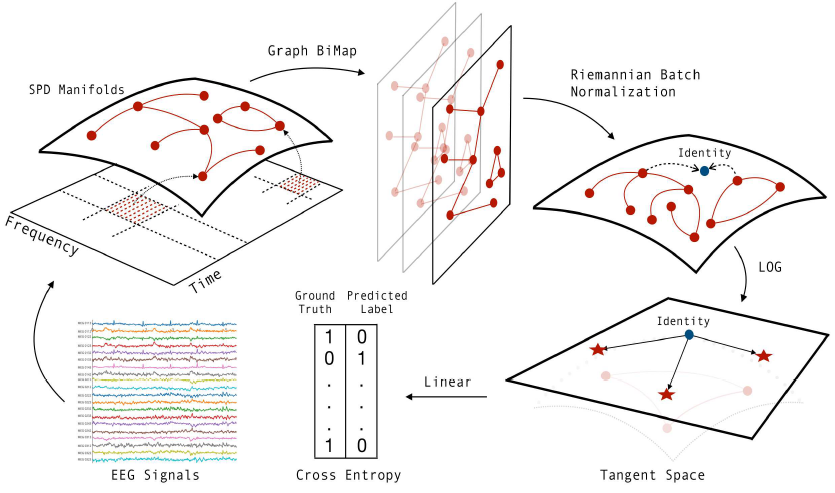
\includegraphics[height = 4cm, width=6.5cm]{images/2023_Ju.png}
	\end{center}
	
	\begin{center}
		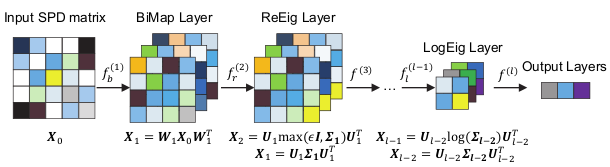
\includegraphics[height = 2.5cm, width=9cm]{images/2017_Huang.png}
	\end{center}
\end{frame}
%%------------------------------------------------
%
%\begin{frame}
%\frametitle{Multiple Columns}
%\begin{columns}[c] % The "c" option specifies centered vertical alignment while the "t" option is used for top vertical alignment
%
%\column{.45\textwidth} % Left column and width
%\textbf{Heading}
%\begin{enumerate}
%\item Statement
%\item Explanation
%\item Example
%\end{enumerate}
%
%\column{.5\textwidth} % Right column and width
%Lorem ipsum dolor sit amet, consectetur adipiscing elit. Integer lectus nisl, ultricies in feugiat rutrum, porttitor sit amet augue. Aliquam ut tortor mauris. Sed volutpat ante purus, quis accumsan dolor.
%
%\end{columns}
%\end{frame}
%
%%------------------------------------------------
%\section{Second Section}
%%------------------------------------------------
%
%\begin{frame}
%\frametitle{Table}
%\begin{table}
%\caption{Table caption}
%\begin{tabular}{l l l}
%\toprule
%\textbf{Treatments} & \textbf{Response 1} & \textbf{Response 2}\\
%\midrule
%Treatment 1 & 0.0003262 & 0.562 \\
%Treatment 2 & 0.0015681 & 0.910 \\
%Treatment 3 & 0.0009271 & 0.296 \\
%\bottomrule
%\end{tabular}
%\end{table}
%\end{frame}
%
%%------------------------------------------------
%
%\begin{frame}
%\frametitle{Theorem}
%\begin{theorem}[Mass--energy equivalence]
%$E = mc^2$
%\end{theorem}
%\end{frame}
%
%%------------------------------------------------
%
%\begin{frame}[fragile] % Need to use the fragile option when verbatim is used in the slide
%\frametitle{Verbatim}
%\begin{example}[Theorem Slide Code]
%\begin{verbatim}
%\begin{frame}
%\frametitle{Theorem}
%\begin{theorem}[Mass--energy equivalence]
%$E = mc^2$
%\end{theorem}
%\end{frame}\end{verbatim}
%\end{example}
%\end{frame}
%
%%------------------------------------------------
%
%\begin{frame}
%\frametitle{Figure}
%\begin{figure}
%\centering
%\includegraphics[width=0.8\linewidth]{figures/example_figure.pdf}
%\end{figure}
%\end{frame}
%
%%------------------------------------------------
%
%\begin{frame}[fragile] % Need to use the fragile option when verbatim is used in the slide
%\frametitle{Citation}
%An example of the \verb|\cite| command to cite within the presentation:\\~
%
%This statement requires citation \cite{p1}.
%\end{frame}
%
%%------------------------------------------------
%
%\begin{frame}
%\frametitle{References}
%\footnotesize{
%\begin{thebibliography}{99} % Beamer does not support BibTeX so references must be inserted manually as below
%\bibitem[Smith, 2012]{p1} John Smith (2012)
%\newblock Title of the publication
%\newblock \emph{Journal Name} 12(3), 45 -- 678.
%\end{thebibliography}
%}
%\end{frame}
%
%%------------------------------------------------
%
%\begin{frame}
%\Huge{\centerline{The End}}
%\end{frame}

%----------------------------------------------------------------------------------------
%   SUPPLEMENTARY SLIDES
%----------------------------------------------------------------------------------------
%\appendix
%
%\begin{frame}{Supplementary figure}
%This slide is not part of total slide count or the navigational panel.
%\begin{figure}
%    \centering
%    \missingfigure{Insert supplementary figure here.}
%\end{figure}
%\end{frame}

%----------------------------------------------------------------------------------------

\end{document} 